\documentclass[12pt]{article}

\usepackage{amsfonts}
\usepackage{amsmath}
\usepackage{geometry}
\usepackage{xcolor,graphicx}
%\usepackage{enumitem}
%\usepackage{wrapfig}
%\usepackage{subcaption}
%\usepackage{hyperref}

\newcommand{\diff}[3][]{\frac{d^{#1}#2}{d{#3}^{#1}}}
\newcommand{\pdiff}[3][]{\frac{\partial^{#1}#2}{\partial{#3}^{#1}}}

%\bibliographystyle{ieeetr}

\newgeometry{margin=1in}
%\setlength\parindent{0pt}

\begin{document}

\begin{figure}[tbp]
\centering
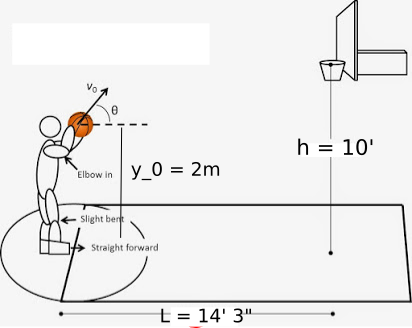
\includegraphics[scale=0.75]{freethrow}
\caption{Diagram of a free throw.}
\end{figure}

\section*{1.5 Scoring a Free Throw}
Starting from $F = ma$ we have
\begin{align*}
m \ddot{y} &= -g m, & y(0) &= y_0, & y(t_{crit}) &= h, & \dot{y} &= v_0 \sin \theta
\end{align*}
in the $y$ direction, and
\begin{align*}
m \ddot{x} &= 0, & x(0) &= 0, & x(t_{crit}) &= L, & \dot{x} &= v_0 \cos \theta
\end{align*}
in the $x$ direction. Integrating these expressions yields
\begin{align}
y &= -\frac{1}{2} g t^2 + v_0 \sin \theta t + y_0, \nonumber \\
x &= v_0 \cos \theta t.
\label{eq:x}
\end{align}
Since $x(t_{crit}) = L$, it must be by \eqref{eq:x} that
\begin{align*}
t_{crit} = \frac{L}{v_0 \cos \theta}.
\end{align*}
From this expression and the fact that $y(t_{crit}) = h$ we obtain
\begin{align*}
h - y_0 = -\frac{1}{2} g \left(  \frac{L}{v_0 \cos \theta} \right)^2 + v_0 \sin \theta \frac{L}{v_0 \cos \theta} + y_0,
\end{align*}
or,
\begin{align*}
v_0 = \left( \frac{2 \cos^2 \theta}{g L^2} \left( y_0 - h + L \tan \theta \right) \right)^{-1/2}.
\end{align*}
Additionally, as the ball enters the hoop $\dot{y} < 0$, and therefore,
\begin{align*}
\dot{y}(t_{crit}) &< 0 \\
-g \frac{L}{v_0 \cos \theta} + v_0 \sin \theta &< 0 \\
v_0^2 \sin \left( 2\theta \right) &< 2gL
\end{align*}
Now, in order to maximize the likelyhood of scoring the free throw we wish to minimize the final velocity. We shall accomplish this by first finding an expression for $v_f$:
\begin{align*}
v_f^2 &= \dot{x}^2 + \dot{y}^2, \\
&= \left( -g t_{crit} + v_0 \sin \theta \right)^2 + \left( v_0 \cos \theta \right)^2, \\
&= \frac{g^2 L^2}{v_0^2 \cos^2 \theta} + v_0^2 - 2 g L \tan \theta, \\
&= 2 g \left( y_0 - h + L \tan \theta \right) + \frac{g L^2}{2 \cos^2 \theta} \frac{1}{y_0 - h + L \tan \theta} - 2 g L \tan \theta, \\
&= 2 g \left( y_0 - h \right) + \frac{g L^2}{2 \cos^2 \theta} \frac{1}{y_0 - h + L \tan \theta}.
\end{align*}
We can now proceed by differentiating with respect to $\theta$ to yield
\begin{align*}
2 v_f \diff{v_f}{\theta} = \frac{g L^2}{2} \left[ 2 \left( \cos \theta \right)^{-3} \sin \theta \left( y_0 - h + L \tan \theta \right)^{-1} + \left( \cos \theta \right)^{-2} \left( -\left( y_0 - h + L \tan \theta \right)^{-2} \right) L \sec^2 \theta \right].
\end{align*}
Which we will now set to 0 and simplify to find\footnote{With the aid of Mathematica.}
\begin{align*}
0 &= \frac{g L^2}{2} \left[ \frac{2 \sin \theta}{\left( \cos \theta \right)^{3}} \frac{1}{y_0 - h + L \tan \theta} - \frac{L}{\left( \cos \theta \right)^4} \frac{1}{\left( y_0 - h + L \tan \theta \right)^2} \right], \\
&= - \frac{gL}{2 \cos^4 \theta} \frac{\cos \left( 2 \theta \right) + \frac{y_0 - h}{L} \sin \left( 2 \theta \right)}{\tan \theta - \frac{y_0 - h}{L}}
\end{align*}
or,
\begin{align*}
\tan \left( 2 \theta \right) &= \frac{- L}{h - y_0} \\
\theta &= \frac{1}{2} \left( \arctan \left( \frac{-L}{h - y_0} \right) + \pi \right).
\end{align*}
Evaluating with typical values, we find $\theta \sim 51.78^\circ$.

\newpage

\section*{3.5 Boating}
We assume the area of the wetted area, $A$, is a function of the number of people, $N$, the volume per person, $V$, and the power generated per person, $P$, then
\begin{align*}
A = f(N, V, P).
\end{align*}
By comparing the units we find
\begin{align*}
L^2 = p^\alpha \left( \frac{L^3}{p} \right)^\beta \left( \frac{M L^2}{T^3 p} \right)^\gamma,
\end{align*}
where $L$ is our length unit, $p$ is our persons unit, $M$ is our mass unit, and $T$ is our time unit. This gives us the system
\begin{align*}
2 &= 3 \beta + 2 \gamma, \\
0 &= \alpha - \beta - \gamma, \\
0 &= \gamma, \\
0 &= -3\gamma.
\end{align*}
Solving this system we find $\alpha = \beta = \frac{2}{3}$, and thus,
\begin{align*}
A \propto \left( NV \right)^{2/3}.
\end{align*}

We can use a similar proceedure for the drag force experienced by the boat by considering the area, as well as the speed of boat, $U$, and the density of the water, $\rho$. By again considering the units, we have
\begin{align*}
\frac{M L}{T^2} = \left( L^2 \right)^\alpha \left( \frac{L}{T} \right)^\beta \left( \frac{M}{L^3} \right)^\gamma.
\end{align*}
Once again we obtain a system from this equation:
\begin{align*}
1 &= \gamma, \\
1 &= 2\alpha + \beta - 3\gamma, \\
-2 &= -2\beta,
\end{align*}
which has the solution $\alpha = 1$, $\beta = 2$, $\gamma = 1$. Therefore,
\begin{align*}
D \propto A U^2 \rho. 
\end{align*}

The total power of the rowers, $NP$, must be proportional to rate at which work is done. The work done is the force multiplied by the velocity. That is, $NP \propto DU$. We then find
\begin{align*}
NP &\propto \left( NV \right)^{2/3} \rho U^3, \\
U^3 &\propto \frac{NP}{\left( NV \right)^{2/3} \rho}, \\
&\propto \left( \frac{NP^3}{V^2 \rho^3} \right)^{1/3},
\end{align*}
and finally,
\begin{align*}
U &\propto \left( \frac{NP^3}{V^2 \rho^3} \right)^{1/9}.
\end{align*}

If $V$ and $P$ are both proportional to mass then it is advantageous to have a larger mass since
\begin{align*}
U &\propto \left( \frac{NM^3}{M^2 \rho^3} \right)^{1/9} \\
&\propto \left( \frac{N}{\rho^3} \right)^{1/9} M^{1/9}.
\end{align*}
However, since it is raised to the power of one ninth, this is relatively negligible.
\end{document}









